\documentclass[12pt,a4paper]{report}
\usepackage[T1]{fontenc}
\usepackage[utf8]{inputenc}
\usepackage{charter}
\usepackage{ngerman}
\usepackage[left=2cm,right=2cm,top=2cm,bottom=2cm]{geometry}
\usepackage{graphicx}
\usepackage{amsmath}
\usepackage{tikz}

\renewcommand\thesection{\arabic{section}.} 

\begin{document}
	\section{Erzwungene Schwingung und elektrische Resonanz}
	Das \dq Weiterlaufenlassen\dq\ eines mechanischen Schwingkreises erhalten wir, wenn wir von außen dem Schwingkreis passenden \dq Anschwung\dq\ geben.
	Das bedeutet, dass die äußere Anregungsfrequenz mit der Eigenfrequenz identisch ist.
	Dies übertragen wir jetzt auf den elektrischen Fall:\\
	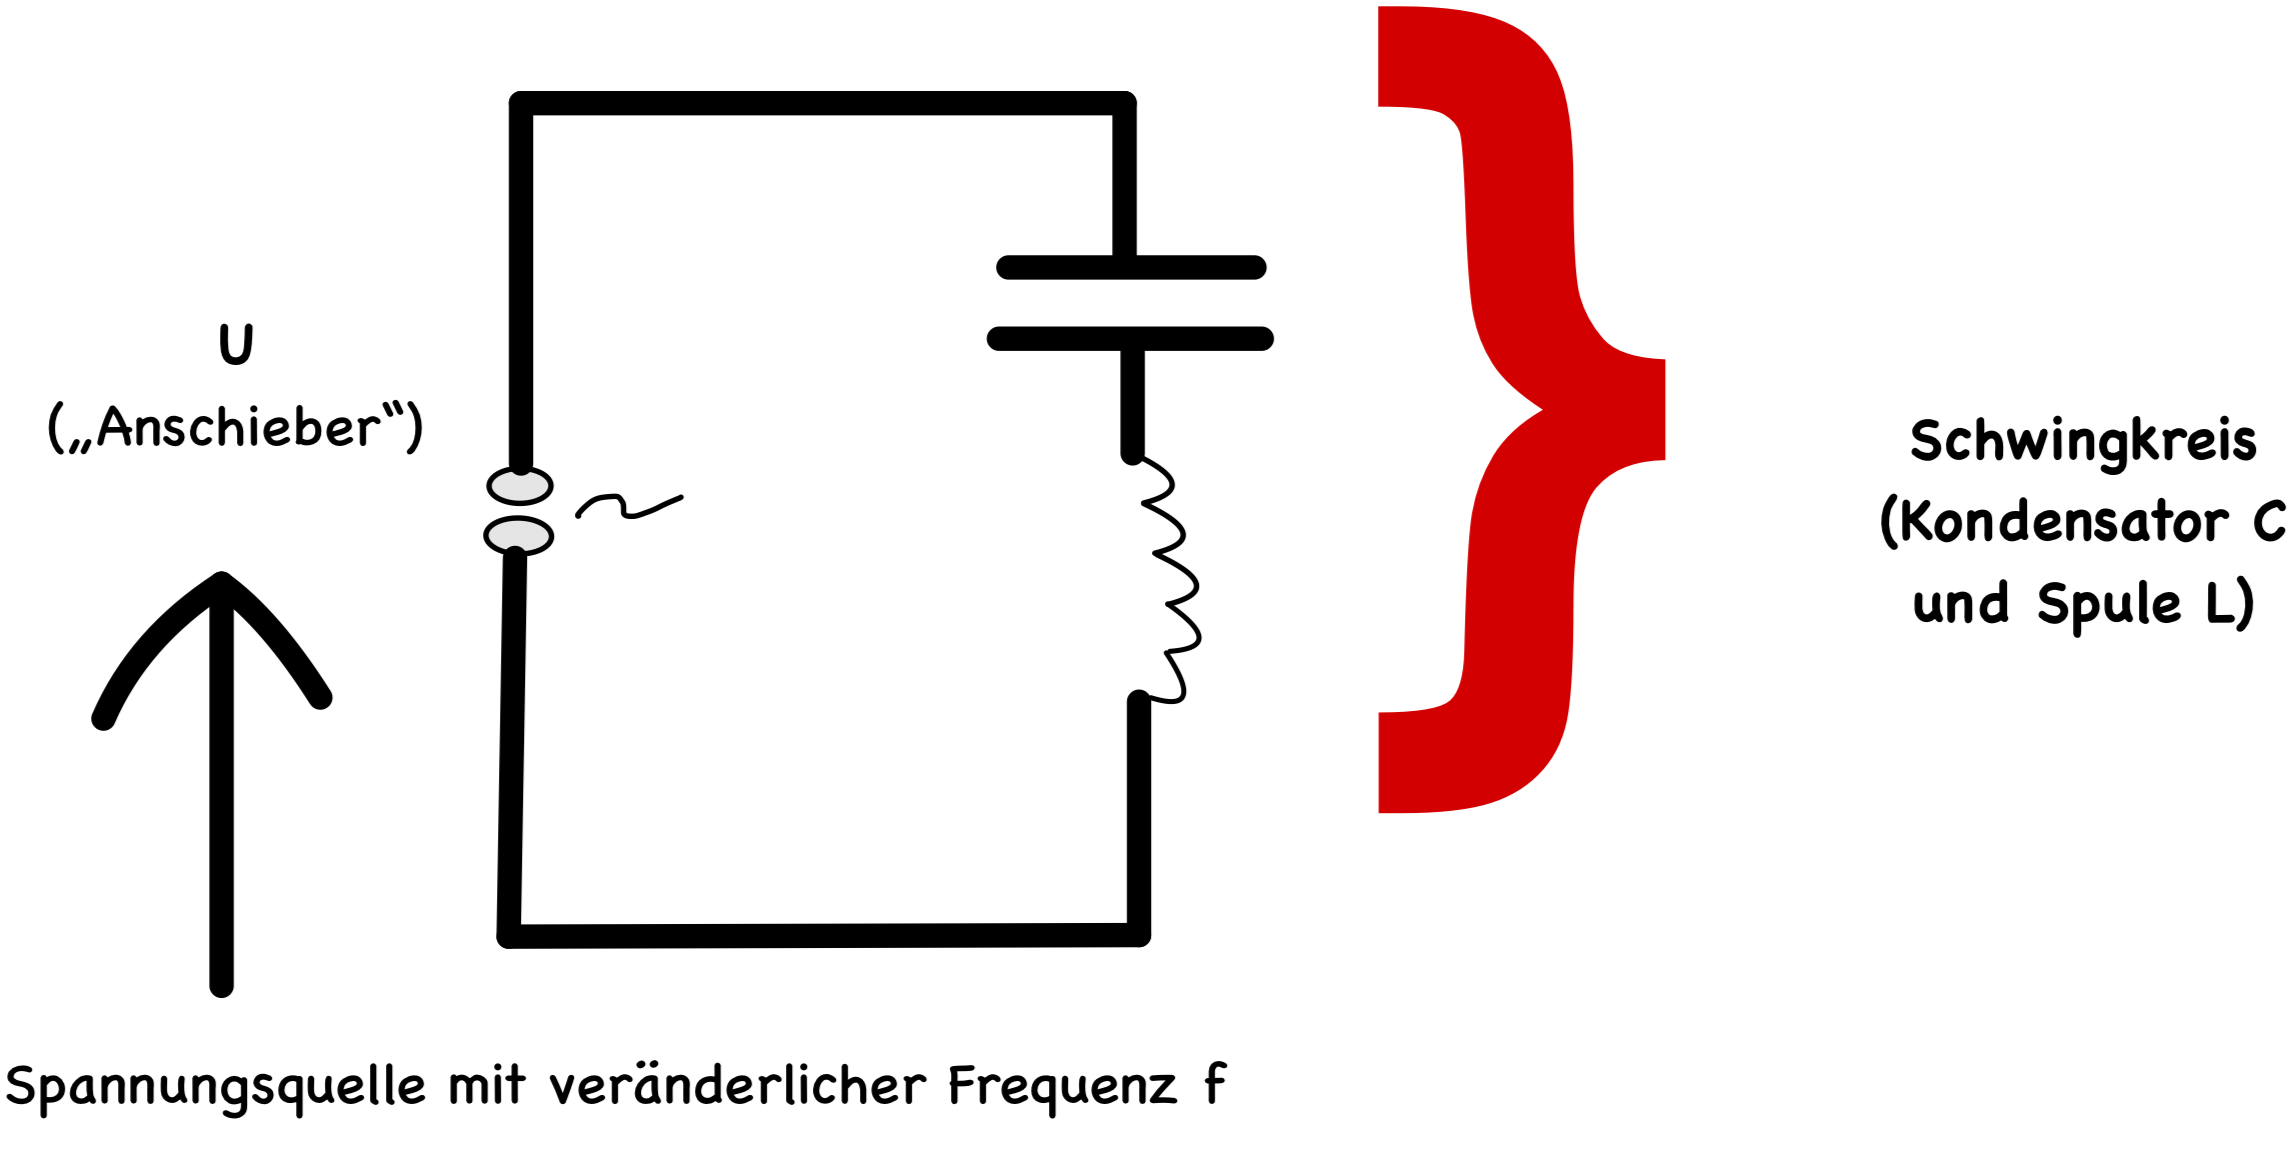
\includegraphics[width=\textwidth]{Image.jpeg.png} \\
	Das Ampermeter zeigt uns nun, wie stark der Schwingungsausschlag ist, wenn wir unterschiedliche Anregungsfrequenzen einstellen.\\
	Betrachten wir nun die Stromstärke $I$ gegen die Anregungsfrequenz, so sehen wir, dass bei einer kleinen Anregungsfrequenz die Stromstärke gering ist.
	Erhöhen wir sukzessive die Frequenz, wird die Stromstärke auch höher, bis wir eine maximale Stärke erreicht haben - dies ist der Fall bei der Eigenfrequenz des Schwingkreises.
	Anschließend fällt die Stromstärke wieder, wenn wir die Frequenz noch weiter erhöhen: \\
	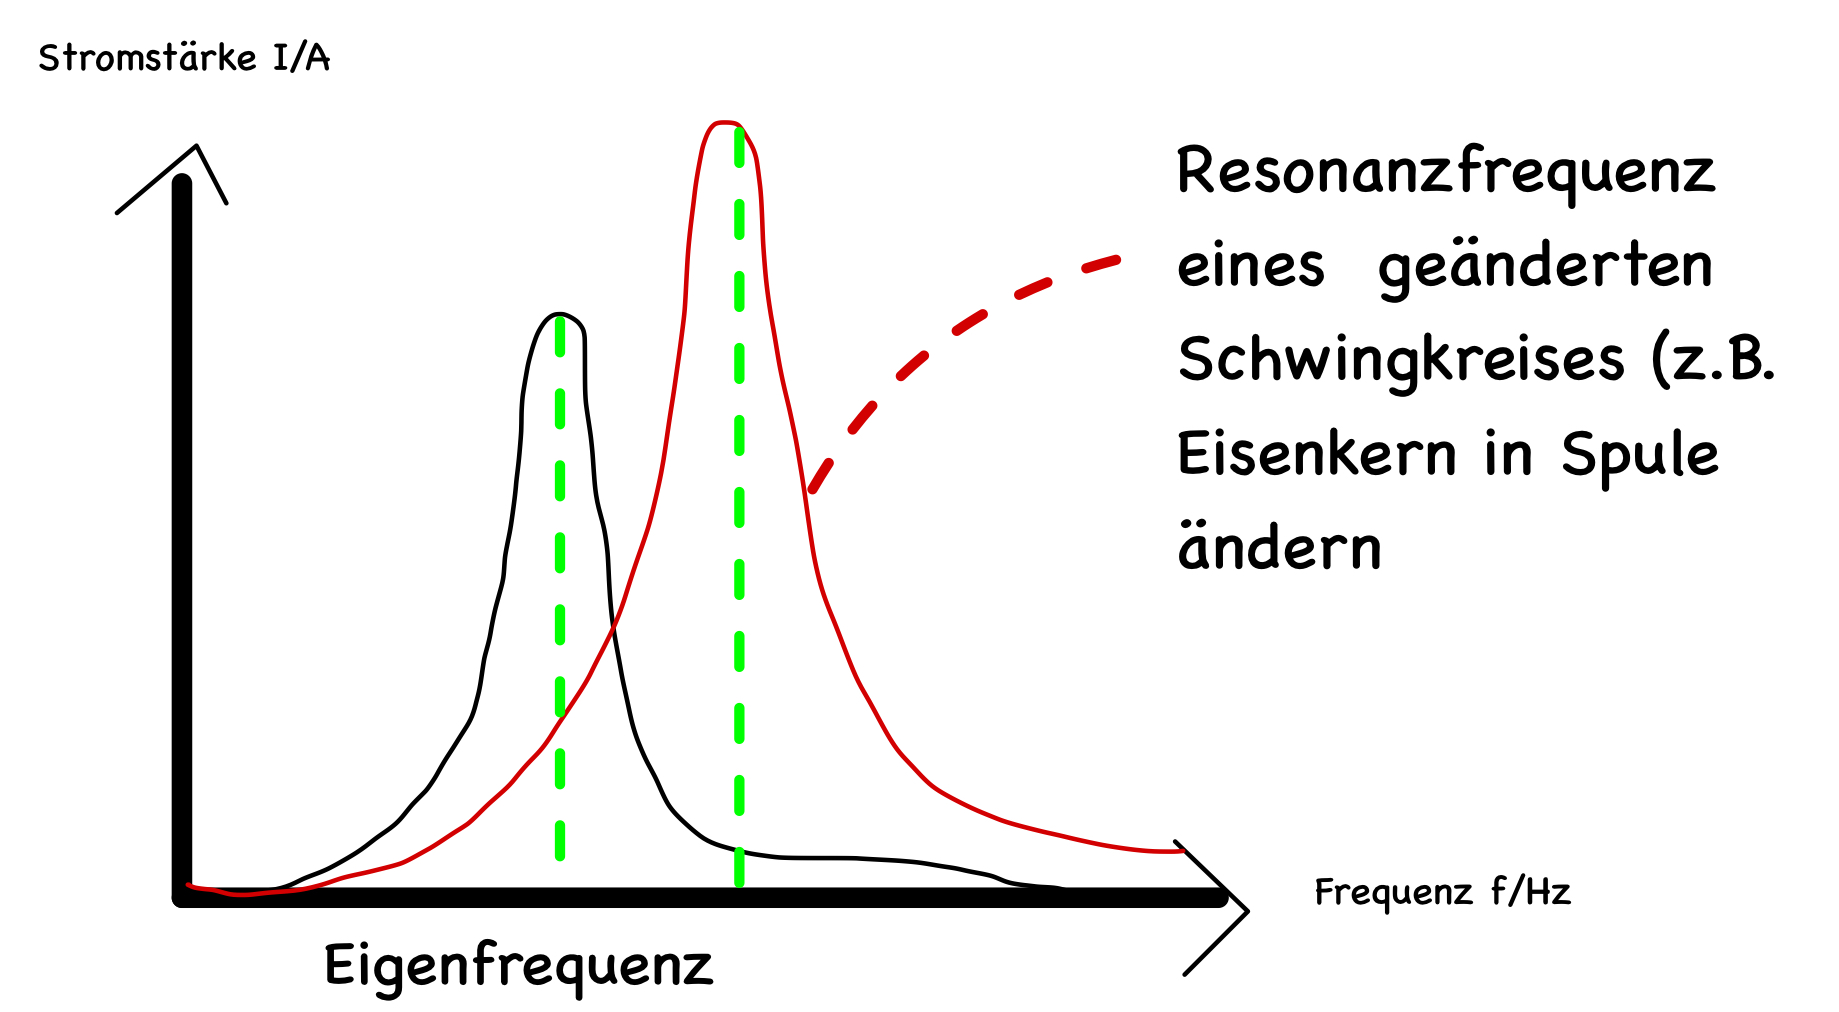
\includegraphics[width=0.75\textwidth]{IMG_1930.jpg}\\
	Hier ist nun die Thomsonsche Schwingungsformel wichtig:\\
	\begin{align*}
		\frac{1}{f_{eigen}} = T_{Eigen} = 2\pi \cdot \sqrt{LC} = T_{Resonanz} = \frac{1}{f_{Resonanz}}
	\end{align*}
\end{document} 